\subsubsection{Discretisation error}
\label{sec:astrodisc}

Due to the use of a discrete time step an error relative to the real solution is induced. By testing the tool with the same initial conditions using different time meshes the difference between the solutions can be analysed. When the smallest time step is assumed to be exact, the error of the larger time steps can be expressed relative to that. This relative error is shown in Figure \ref{fig:atmos_disc}. Please also note these errors are calculated running the tool without active control.

Two conclusions can be drawn from this. First the error decreases quadratically with decreasing time step. This means that the system converges. Secondly the error is smaller than $1 \left[m\right]$ for a time step smaller than $0.3 \left[s\right]$. This error is negligible compared to the error that will be induced by the assumptions that were made in Section \ref{sec:astroassumption}.

%Initial Position
%rx = -4143775;
%ry = 10*R_m;
%R = [rx,ry,0];

%Initial Velocity
%v = 7.1679e+03; %[m/s]
%V = [0,-v,0];

\begin{figure}[ht]
	\centering
	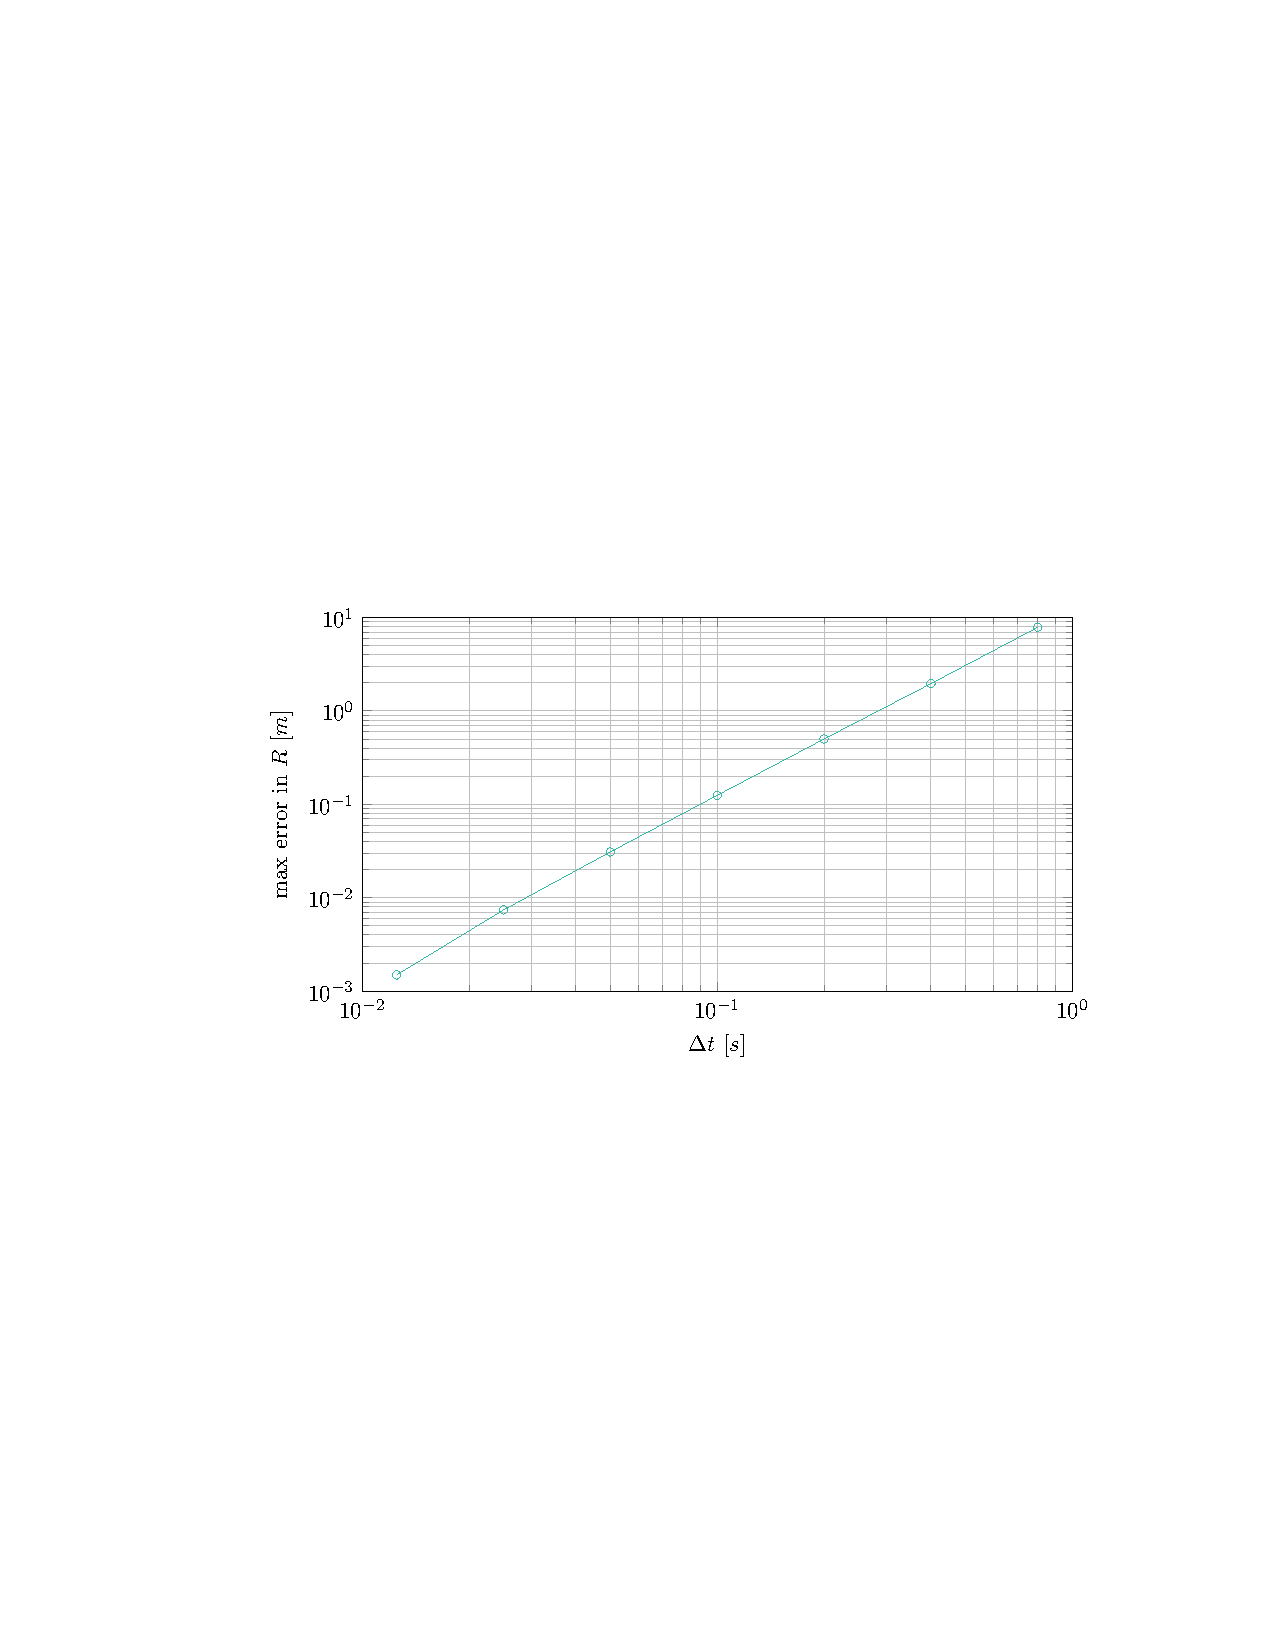
\includegraphics[width=0.8\textwidth]{Figure/orbit/dicretization.pdf}
	\caption[Discretisation error in location $\left(\gls{sym:Rv}\right)$ after one pass through the atmosphere for the rigid shape]{Discretisation error in radius $\left(\gls{sym:Rv}\right)$ after one pass through the atmosphere for initial position $\left[-4\mbox{ }143\mbox{ }775,10\cdot\gls{con:rm}\right] \left[m\right]$ and initial velocity $\left[0,-7167.9\right] \left[m\cdot s^{-1} \right]$ at $\gls{sym:alpha}=-10 \left[deg\right]$ for the rigid shape}
	\label{fig:atmos_disc}
\end{figure}

\subsubsection{Verification through comparison with Kepler orbit}
\label{sec:astroverf}

In this section the results from the numerical simulation, which is usually only used in atmosphere, is compared to a Kepler orbit. For this comparison the density is assumed to be zero, or in other words, it is assumed that there is no atmosphere. This comparison is done for different values of $\Delta t$. The error for each $\Delta t$ is shown in Figure \ref{fig:kep_error}.

\begin{figure}[ht]
	\centering
	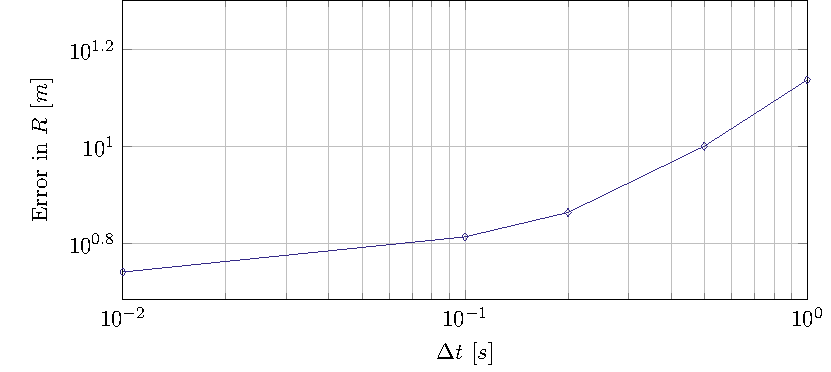
\includegraphics[width=0.8\textwidth]{Figure/orbit/num_kep.pdf}
	\caption[Error compared to a Kepler orbit]{Error compared to a Kepler orbit after $50\mbox{ }005 \left[s\right]$ for initial position $\left[-4\mbox{ }143\mbox{ }775,10 \cdot \gls{con:rm} \right] \left[m\right]$ and initial velocity $\left[0,-7167.9\right] \left[m\cdot s^{-1} \right]$ at $\gls{sym:alpha}=-10 \left[deg\right]$ for the shape of the rigid concept}
	\label{fig:kep_error}
\end{figure}

The figure shows the error is between 15 and 5 for $\Delta t$ between 1 and 0.01. The error decreases, but seems to tend to a non-zero constant value. The method used for numerical simulation is thus convergent, but has a small offset from the exact solution. This error is however so small it can easily be accepted. It should also be noted that the numerical simulation is never ran longer than 2000 seconds during the entire mission trajectory calculation. The error calculated here is thus much larger than the error in the actual calculations will be.

\subsubsection{Validation}
\label{sec:astroval}

Validation for a mission as unique as this one is difficult as no reference data is available. Testing is thus the only method to do any validation of the model. Because of budget and time constraints of the conceptual design, testing is not possible. Engineering gut feeling is now the only way to get an idea of the correctness of the model. No final conclusions can be drawn from this, and thus no conclusion will be drawn.